\documentclass{beamer}
\mode<presentation>
\usetheme{CambridgeUS}
\usepackage[russian]{babel}
\usepackage[utf8]{inputenc}
\usepackage[T2A]{fontenc}
\usepackage{sansmathaccent}

\usepackage{verbatim}
\usepackage{alltt}

\pdfmapfile{+sansmathaccent.map}
\title[Типизированные файлы]{Типизированные файлы}
\author{Наумов Д.А., доц. каф. КТ, ИТГД }
\date[04.05.2020] {Программирование и алгоритмические языки, 2020}

\begin{document}

%ТИТУЛЬНЫЙ СЛАЙД
\begin{frame}
  \titlepage
\end{frame}
  
%СОДЕРЖАНИЕ ЛЕКЦИИ
\begin{frame}
  \frametitle{Содержание лекции}
  \tableofcontents  
\end{frame}
  

\section{Файловый тип данных}

\begin{frame}
\begin{block}{Файл}
именованная сущность, для которой определены операции ввода и вывода данных.
\end{block}
Для работы с файлами в Pascal предусмотрены \textbf{файловые типы данных}:
\begin{enumerate}
\item типизированные: информация считывается и записывается в переменные конкретного типа (целые, вещественные, массивы и т. д.);
\item нетипизированные: информация считывается и записывается блоками определённого размера.
\item текстовые: информация обрабатывается посимвольно, но возможно чтение и запись данных в переменные строкового, целого и вещественного типа.
\end{enumerate}
В данной лекции будут рассматриваться \textbf{типизированные файлы}.
\end{frame} 

\begin{frame}[fragile]{Описание переменной файлового типа}
\begin{alltt}
 1 type
 2   TElem = real; 
 3   TPersonInfo = record
 4      Name: string[25];
 5      Age: integer;
 6      Birth: record
 7        Day: 1..31; Month: 1..12; Year: integer;
 8     end;
 9   end;
 10  TValueFile = file of TElem; 
 11  TPersonFile = file of TPersonInfo; 
 // описание переменных файлового типа
 12 var                  
 13   F1: TValueFile;  //тип элементов - TElem, т.е. real
 14   F2: TPersonFile; //тип элементов - TPersonInfo  
 15   F3: file of integer; //тип элементов - integer
\end{alltt}
\end{frame}

\section{Операции с файлами}
\subsection{Процедура Assign}
\begin{frame}[fragile]{Assign}
\begin{block}{Процедура Assign}
связывает файловую переменную с файлом.
\end{block}
Синтаксис: Assign(f, s)
\begin{itemize}
\item f - переменная файлового типа;
\item s - строка, полный или частичный путь к файлу. 
\end{itemize}
\begin{alltt}
 1 var                  
 2   F1, F2: file of real;
 3 begin
 4   Assign(F1, 'myfile.dat');
 5   Assign(F2, 'c:\textbackslash work\textbackslash myfile.dat');
\end{alltt}
\end{frame} 

\subsection{Процедуры Rename, Erase}
\begin{frame}[fragile]{Rename, Erase}
\begin{block}{Процедура Rename}
переименовывает или перемещает не открытый файл.
\end{block}
Синтаксис: Rename(f, s)
\begin{itemize}
\item f - переменная файлового типа;
\item s - строка, полный или частичный путь к файлу. 
\end{itemize}
\begin{block}{Процедура Erase}
удаляет не открытый файл.
\end{block}
Синтаксис: Erase(f)
\begin{itemize}
\item f - переменная файлового типа.
\end{itemize}
\end{frame} 

\subsection{Процедуры открытия файла}
\begin{frame}[fragile]{Открытие файла}
После установления связи между файловой переменной и именем файла на диске нужно открыть файл, воспользовавшись процедурами reset, или rewrite.
\begin{block}{Процедура Reset}
открывает файл для чтения.
\end{block}
Синтаксис: Reset(f)
\begin{itemize}
\item f - переменная файлового типа.
\item файл должен существовать (иначе - ошибка ввода-вывода);
\item текущей позицией для чтения становится начало файла.
\end{itemize}
\begin{alltt}
 1 var                  
 2   F1: file of real;
 3 begin
 4   Assign(F1, 'myfile.dat');
 5   Reset(F1);
\end{alltt}
\end{frame} 

\begin{frame}[fragile]{Открытие файла}
\begin{block}{Процедура Rewrite}
открывает файл для записи.
\end{block}
Синтаксис: Rewrite(f)
\begin{itemize}
\item f - переменная файлового типа.
\item содержимое файла уничтожается;
\item \textbf{текущей позицией} для чтения становится начало файла.
\end{itemize}
\begin{alltt}
 1 var                  
 2   F1: file of real;
 3 begin
 4   Assign(F1, 'myfile.dat');
 5   Rewrite(F1);
\end{alltt}
\textbf{Указатель текущей позиции} - место в файле, с которого будет осуществляться процедура чтения или записи.
\end{frame} 

\subsection{Процедура закрытия файла}
\begin{frame}[fragile]{Закрытие файла}
Процедуры записи в файл записывают информацию в буфер. После того как буфер заполнится, вся информация из него переносится в файл. При выполнении процедуры \textit{Close} сначала происходит запись буфера файла на диск, и только потом файл закрывается.
\begin{block}{Процедура Close}
закрывает файл.
\end{block}
Синтаксис: Close(f), f - переменная файлового типа.
\begin{alltt}
 1 var F1: file of real;
 2 begin
 3   Assign(F1, 'myfile.dat');
 4   Rewrite(F1);
 5   Write(F1, Pi);
 6   Close(F1);
 7 end.
\end{alltt}
\end{frame} 

\subsection{Чтение и запись в файл}
\begin{frame}[fragile]{Чтение из файла}
\begin{block}{Процедура Read}
выполняет чтение информации из файла.
\end{block}
Синтаксис: Read(f, x1, x2, x3, $...$, xn);
\begin{itemize}
\item f - переменная файлового типа;
\item x1, x2, x3, $...$, xn - переменные.
\end{itemize}
Для типизированных файлов тип переменной должен совпадать с типом компонент файла.
\begin{alltt}
 1 var F1: file of real; 
 2 var v: real; 
 3 begin
 4   Assign(F1, 'myfile.dat');
 5   Reset(F1);
 6   Read(F1, v); //считываем одно число
 7   Write(F1, v); //выведем его на экран
 8   Close(F1);
 9 end.
\end{alltt}
\end{frame} 

\begin{frame}[fragile]{Запись в файл}
\begin{block}{Процедура Write}
выполняет запись информации в типизированный файл.
\end{block}
Синтаксис: Write(f, x1, x2, x3, $...$, xn);
\begin{itemize}
\item f - переменная файлового типа;
\item x1, x2, x3, $...$, xn - переменные.
\end{itemize}
Для типизированных файлов тип переменной должен совпадать с типом компонент файла.
\begin{alltt}
 1 var F1: file of real; 
 2 var i: integer;
 3 begin
 4   Assign(F1, 'myfile.dat');
 5   Rewrite(F1);
 6   for i := 1 to 10 do 
 7     Write(F1, random());  
 8   Close(F1);
 9 end.
\end{alltt}
\end{frame} 

\subsection{Проверка достижения конца файла}
\begin{frame}[fragile]
\begin{block}{Функция Eof}
возвращает True, если при чтении из файла был достигнут конец файла.
\end{block}
Синтаксис: Eof(f)
\begin{itemize}
\item f - переменная файлового типа
\end{itemize}
Пример: чтение всех данных из файла.
\begin{alltt}
 1 var F1: file of real; 
 2 var v: real;
 3 begin
 4   Assign(F1, 'myfile.dat');
 5   Reset(F1);
 6   while not EOF(F1) do 
 7   begin
 8     Read(F1, v);  
 9     Writeln(v); 
 10  end;
 8   Close(F1);
 9 end.
\end{alltt}
\end{frame}

\subsection{Подпрограммы работы с типизированными файлами}
\begin{frame}
\begin{block}{Функция Filesize(f)}
возвращает для открытого типизированного файла \textbf{f} количество его компонент.
\end{block}
\begin{block}{Функция Filepos(f)}
возвращает текущую позицию (чтения, записи) в открытом файле \textbf{f}.
\end{block}
\begin{block}{Процедура Seek(f, k)}
устанавливает указатель в открытом файле, связанном с файловой переменной \textbf{f}, на компонент с номером \textbf{k} (нумерация компонентов идет от 0).
\end{block}
\begin{block}{Процедура Truncate(f)}
отсекает часть открытого файла, начиная с текущего компонента, и подтягивает на его место
конец файла.
\end{block}
\end{frame}

\subsection{Контроль ошибок ввода-вывода}
\begin{frame}[fragile]{Контроль ошибок}
При открытии файла и чтении данных осуществляет контроль ошибок ввода-вывода. Если произошла ошибка (открываемый для чтения файл не существует), то проверка может осуществляться через обращаение к функции IOResult.
\begin{alltt}
 1 Assign(F, 'unexist.file');
 2 \{\$I+\}
 3 Reset(F);
 4 \{\$I-\} 
 5 if IOResult = 0
 6 //файл существует 
 7 else
 8 //произошла ошибка ввода-вывода
\end{alltt}
\end{frame}

\begin{frame}
\begin{block}{Коды ошибок операций ввода-вывода}
\begin{center}
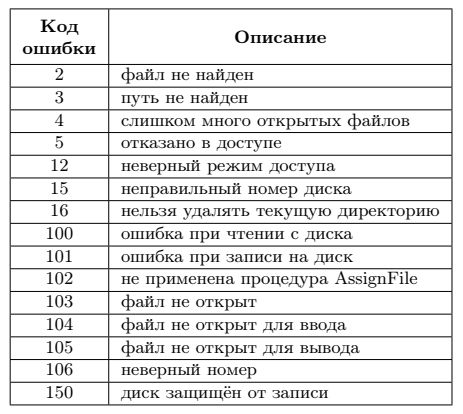
\includegraphics[scale=0.6]{images/ioresult.png}
\end{center}
\end{block}
\end{frame}

\end{document}
